\section{Adaptation Models}
\label{sec:adaptation_models}
%------------------------------------------------------------------------- 

Before introducing the analysed adaptation models, a terminology review is
given taking into account the differences between adaptable and adaptive
defined by \citeauthor{fischer_user_2001} (see these definitions in 
Section~\ref{sec:definitions}). \\

\citet{fischer_user_2001} defined \textit{adaptive} and \textit{adaptable} 
principles in 2001 through 6 different concepts: definition, knowledge, strengths, weaknesses, required mechanisms, and application domains. 
Table~\ref{tbl:fischer} shows a representation of these concepts.

\begin{table}
 \caption{~\citet{fischer_user_2001} comparison between adaptable and adaptive systems.}
 \label{tbl:fischer}
 \footnotesize
 \centering
\begin{tabular}{l l l}
  \hline
			& \textbf{Adaptive} 			& \textbf{Adaptable}\\
  \hline
	Definition	& Dynamic adaptation by the system  	& User changes (with substantial system	\\
			& itself to current tasks and current user.& support) the functionality of the system\\
	Knowledge	& Contained in the system; projected in & Knowledge is extended.		\\
			& different ways.			& ~					\\ 
	Strengths	& Little (or no) effort by the user; no & User is in control; user knows her/his\\
			& knowledge of the user is special required.& task best; system knowledge will fit \\
			& 					& better; success model exists.		\\
	Weaknesses	& User has difficulty developing a coherent& Systems become incompatible; user must\\
			& model of the system; loss of control;	few & do substantial work; complexity is \\
			& (if any) success models exist (except	& increased (user needs to learn the 	\\
			& humans).				& adaptation component). 		\\
	Mechanisms	& Models of users, tasks, and dialogs;	& Layered architecture; domain models 	\\
	required	& knowledge base of goals and plans;  	& and domain-orientation; back-talk from\\
			& powerful matching capabilities;  	& the system; design rationale.		\\
			& incremental update of models.		& ~ 					\\
	Application	& Active help systems, critiquing systems,& Information retrieval, end-user	\\
	domains		& differential descriptions, user interface& modifiability, tailorability, 	\\
			& interface customization, information	& filtering, design in use.		\\
			& retrieval.				& ~					\\
  \hline
\end{tabular}
\end{table}

As is shown in Table~\ref{tbl:fischer}, an adaptive system is able to dynamically 
change due if a certain situation is met. This situation might act as a trigger
for the adaptation. Adaptable systems, however, require the user intervention. 
Current smartphones provide a set of tools to allow users to adapt several 
elements of the user interface. For example, font sizes, colour combinations, 
screen magnification and dictation are several adaptable functionalities available 
in such devices\footnote{http://developer.android.com/guide/topics/ui/accessibility/index.html}\footnote{https://www.apple.com/accessibility/ios/},
known as accessibility tools. Figure~\ref{fig:accessibility_ios} shows an example 
of several accessibility tools in iOS, including VoiceOver\footnote{https://www.apple.com/accessibility/ios/voiceover/}
on the left and Siri\footnote{https://www.apple.com/ios/siri/} on the right.

\begin{figure}
\centering
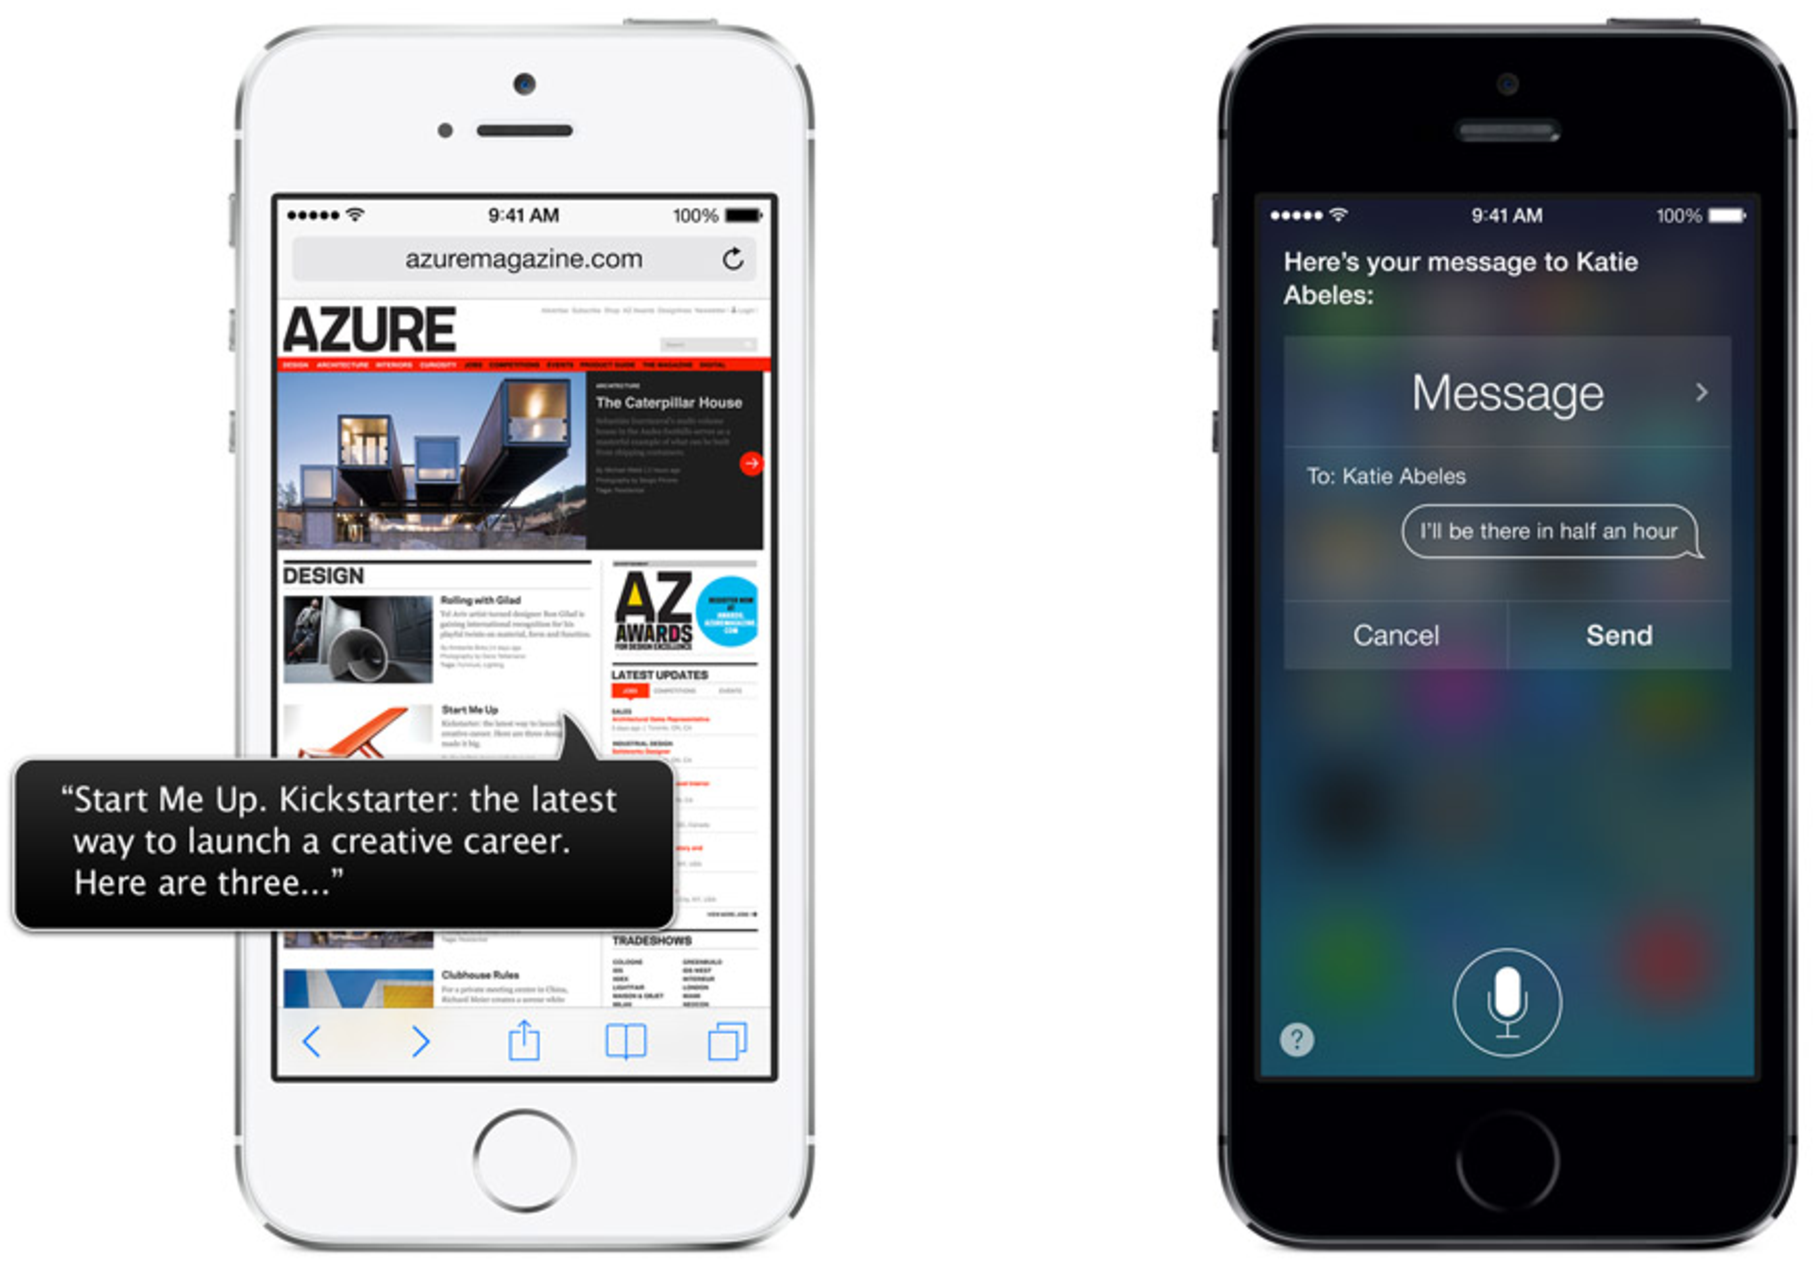
\includegraphics[width=0.7\textwidth]{accessibility_ios.pdf}
\caption{iOS VoiceOver and Siri.}
\label{fig:accessibility_ios}
\end{figure}

These accessibility functionalities make the user interfaces \textit{adaptable}
by the users. On the contrary, \textit{adaptive} user interfaces would modify 
the aspect of the shown elements without the user intervention. This means that 
adaptable user interfaces needs the user to change the corresponding adaptable 
characteristic (e.g., the font size) while an adaptive user interface would 
adapt without it.

Subsequently, \textit{adaptivity} and \textit{adaptability} are introduced. 
\textit{Adaptivity} is related to the fact that a system or a service is able to 
learn somehow to change itself to increase the user satisfaction in the interaction 
process. On the other hand, \textit{adaptability} deals with the property of the 
system or service to be customized by the user~\citep{jameson_modelling_2001}.

Now that we have defined what adaptivity means, several significant adaptive 
systems are presented in the following lines.

\subsection{Significant Adaptation Models}
\label{sec:significant_adaptation_models}

User interface adaptation has evolved through \ac{hci} history. First, and 
dealing with the concept of adaptability (and not adaptivity), user interfaces 
start to be malleable. Colour palettes and screen resolution tools were given to 
the user. Nowadays, regarding our portable devices, even automatic brightness 
control systems are available. Since many years, developers have attempted to 
offer customization tools to the end user. These tools have grown in complexity, 
covering a wider range of functionalities and also users. What is more, a few 
years ago the context was taken into account as the set of characteristics that 
define a situation (the context definition which is adopted in this dissertation
is given by \citet{dey_understanding_2001}, and its definition is introduced
in Section~\ref{sec:definitions}).

Systems personalization and environment components adaptation have been demonstrated
to benefit both users and service providers~\citep{kobsa_generic_2001}. However, for
achieving a satisfactory adaptation it is necessary to have several inputs, for example,
a user characteristics model. Hence, the service provider will be able to apply the
corresponding adaptations for the corresponding user. Besides, we believe that current
context conditions~\citep{jameson_modelling_2001} and user's device capabilities are also
crucial within this domain. 
% In Section~\ref{sec:interaction_entities} we dig in
% this idea.

\citet{nilsson_model_based_2006} considered that designing user interfaces for
mobile devices tends to be problematic for several reasons (e.g., screen size is
small and interaction mechanisms are very different from a desktop system). Besides,
these devices are usually used in dynamic environments (i.e., variations in the
context). 

% In the literature several context based user interface adaptation solutions can 
% be found. Before reviewing them, it is necessary to first formally define context.
% According to \citet{weerawarana_bean_2001} and \citet{dey_understanding_2001} 
% context is defined as any situation that can be used to characterize the situation 
% of an entity, taking an entity as a person, a place, or an object that is considered
% relevant to the interaction between the user and the application (see
% Section~\ref{sec:context}). The definition of \textit{use context} inherits from
% the context definition itself as the set of variables values which models the
% used device, so as the physical and social environment where the interaction is
% being performed.

\citet{calvary_plasticity_2002} stated in 2002 that a user interface is \textit{plastic}
if it is capable to adapt itself taking into account context changes keeping
the usability. They presented a process and a dynamic software mechanism which
supports context variability. This work was supported by the idea that context
changes may provoke the triggering of several reactions under a \textit{prologue-action-epilogue}
paradigm. 
% In addition, to enhance the performance they introduced a
% \textit{historical of contexts}. By selecting pre-known configurations the
% adaptation process resulted faster. This historical database stores several
% context situations and the corresponding computed reactions. Besides, the
% \textit{''Plasticity Threshold"} and \textit{``Context Coverage"} novel concepts
% help to set the boundaries of a still valid user interface~\citep{calvary_supporting_2001}.

Using another paradigm,~\citet{lehtonen_dynamic_2002} detailed a tool to perform
dynamic adaptation on documents based on several user parameters (language,
document type, and so on). The presented approach is based on several \textit{configuration
files} (Product Configuration Files) which describe the current user interface and
store the user preferences. The user interfaces are designed with Bean Markup
Language~\citep{weerawarana_bean_2001} (a language focused on user interfaces)
and Java Beans.

Following a \textit{middleware} based approach, four remarkable solutions are
highlighted in the following lines. \citet{repo_facilitating_2004} introduced in 
2004 a model that allows the use of Web-based user interfaces (as well as the 
creation of new ones) that covers the environment adaptability requirements and 
context in the best possible way. The main problem is given by the range of 
devices that users typically employ, which have different capabilities and run 
different platforms. This situation causes the need of more flexible applications 
and devices. \citeauthor{repo_facilitating_2004} identified a lack of attention in the initial adaptation process 
(e.g., when the capabilities of the mobile device are identified). This approach 
was based on a \textit{middleware} architecture, and it was capable of detecting 
new devices in the current environment (context changes). It allowed services to 
query for devices' capabilities through a middleware architecture. Once a service 
identified a certain device, it sent the corresponding user interface. 

\citet{nilsson_model_based_2006} introduced a \textit{middleware} solution
which was able to build auto-adaptable systems. In this case, the middleware 
leads the adaptation process dynamically, providing several mechanisms to: 
detect changes in the application context, reason about these changes, and adapt 
to them by a dynamic reconfiguration of the current application. 

Based on the same architecture introduced by~\citet{nilsson_model_based_2006},
\citet{hallsteinsen_self_adaptation_2004} presented a system which was able to 
react to context changes recommending alternative configurations in each case.
The benefit for the user comes from the reasonable adaptation decisions took 
by the middleware, being the developer responsible for describing configuration 
options for important variation points.

\citet{stuerzlinger_user_2006} focused their work on desktop applications
adaptations and on the adaptation, reconfiguration and combination of user
interfaces using a \textit{User Interface Facades} system. Based on the definitions
laid down by~\citet{marmolin_medium_1995}, where differences between superficial
personalization (which allows users to select different options between some
predefined) and deep customization (which allows customizing deeper aspects of
the system) were introduced, authors stated the following criteria for adaptive
interfaces:

\begin{itemize}
  \item Fast, simple, or just-in-time customization: users are able to customize
  their interfaces without advanced planning, whenever they need it, and they will
  be able to do it in a simple way.
  \item Not only big personalization, also local ones (at minor scale).
  \item Deep personalization: users can define new customization rules.
  \item Cross-application personalization: interfaces customization must enable 
  different applications to be combined.
\end{itemize}

A \textit{framework} based approach is presented by~\citet{almeida_imhotep_2011}
in 2011. Imhotep is a framework for user interface adaptation based on inserting
preprocessor primitives within the source code. Thus, at compilation time
different versions of the final application are generated due to the corresponding
user and device parameters. A \ac{wurfl}\footnote{http://wurfl.sourceforge.net/} 
database was used for modelling devices and their capabilities. \ac{wurfl} is a 
\ac{ddr}, a catalogue of mobile device information and a framework for adaptation 
of mobile user interfaces. By using it, authors ensure to have the latest devices 
with their capabilities. As configuration files, the platform checks both user 
and device capabilities and uses them to compile the corresponding solution. This 
approach has the limitation of being static. This means that each change in the 
user capabilities needs a new compilation of the whole application. As this
framework has supposed our first incursion in the field of \acp{aui}, further
details of its main characteristics and architecture are given in Section~\ref{sec:background_imhotep}
and Section~\ref{sec:imhotep_comparison}. Besides, several experiments are
carried out comparing Imhotep and the proposed solution, which will be depicted
in the following chapters.

\citet{evers_achieving_2012} tackle the problem of the need of user interaction 
in the adaptation process. Centred in users, authors discuss about adaptation 
and usability defining different types of adaptation (i.e., forward and backward) 
and different user ways of interaction (i.e., implicit and explicit). This 
perspective helps developers to take into account not only technical 
characteristics (e.g., users models, devices capabilities, context parameters, 
adaptation engines, and so on) but also some psychology to be aware of user mood 
or stress. In stressful situations users may not be comfortable with an adaptation 
engine which asks questions about the process.

Several ideas of the reviewed works are taken into account for the proposed user 
model in combination with the~\citet{casas_user_2008} research. For instance,
the visual handicap metrics in the sensory layer gives an idea of modelling
not the user disability but the minimum needed configuration for a view component
in the screen. This issue is deeply discussed in Section~\ref{sec:user}.

\subsection{Physical Adaptive systems}
\label{sec:pyshical_adaptive_sistems}

Although it is out of the scope of this dissertation, there is a research
pathway dealing with physical adaptive systems. In Tactus\footnote{\url{http://tactustechnology.com/}}, a
company which aims to redefine devices and user experiences by combining the 
modern and traditional interfaces and on-demand buttons on touch
screens for a tactile experience\footnote{\url{https://www.linkedin.com/company/tactus-technology}}, a novel adaptive
technology has been developed. This technology allow screens to dynamically build
physical buttons into a flat touch screen, depending on the current task. For example,
if the user needs to send an email, the keyboard emerges from the screen
as a physical interface. This interface is supported by the combination of
small fluid channels which are routed throughout the Tactile Layer. This layer
enables fluid to expand the top polymer layer to create the physical
buttons\footnote{\url{https://www.youtube.com/watch?v=t4eh-Cn3Pzk}} (see
Figure~\ref{fig:tactus}).

\begin{figure}[H]
\centering
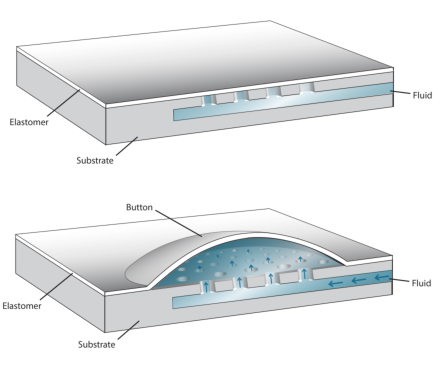
\includegraphics[width=0.55\textwidth]{tactus.pdf}
\caption{Buttons during the flat state (up) and during the raised state (down) in Tactus.}
\label{fig:tactus}
\end{figure}

Nowadays, this technology might be surprising for the reader. Nevertheless, there
are examples of physical user interfaces adaptation all around us. One of the most
common and spread example is shown in cars. The cars companies deal with adaptivity
for the current driver not just inside the car, but also outside. Some models
adapt the driving wheel in depth and height depending on the driver who unlocks
the door. Displays and controller brightness, and radio volume can be also
adapted considering context light or noise. Even the car lights system adapts
to the road conditions.

These are just a few examples of what adaptation technologies might be pointing 
at for the near future.

% ----------------------------------------------------------------------

